\documentclass[14pt,a4paper]{extarticle}
\usepackage[utf8]{inputenc}
\usepackage[english]{babel}
\usepackage{amsmath}
\usepackage{mathtools}
\usepackage{multirow}
\usepackage{subfigure}
\usepackage{amsfonts}
\usepackage{amssymb}
\usepackage{graphicx}
\usepackage{wrapfig}
\usepackage{tabularx}
\usepackage{alphalph}
\renewcommand*{\thesubfigure}%
}%
\DeclarePairedDelimiter\floor{\lfloor}{\rfloor}
\usepackage{float}
\usepackage[export]{adjustbox}

\usepackage[left=2cm,right=2cm,top=4cm,bottom=4cm]{geometry}
\title{A JPEG-like coding system for color images}
\author{Multimedia Coding Course}
\date{Giovanni Gallinaro}
\begin{document}
\maketitle

\section{Introduction}
\subsection{Brief overview of the JPEG coding standard}

The JPEG (Joint Photographic Experts Group) image coding standard is a widely used technique for lossy compression of digital images which has been introduced in 1992. Its popularity is mainly due to the fact that the amount of compression can be adjusted manually, thus allowing a selectable tradeoff between storage size and image quality.

The algorithm works particularly well for full-color highly detailed photographs, since it allows to preserve good quality even with high compression ratios. Conversely, it is not suitable for vector images, text, line art and other image types with sharply-defined lines, since for such images it brings up visibile artifacts and distorts the original shape (some parts of the image could become noticeably blocky). Also, JPEG is not suitable for multiple edits and it does not allow trasparency unlike other formats such as PNG, GIF, BMP, etc.

\subsection{Objective}

The objective of this project is to build a coding system similar to the JPEG algorithm and compare it with the standard JPEG approach.

\section{Technical approach}
\subsection{Details on the JPEG standard}
In this section the technical details on how to implement the JPEG algorithm are reported. After that, I will discuss how the problem has been dealt with in MATLAB.

The first step consists in padding the input image and converting it from RGB to the YCbCr color space. Then, the image is divided into blocks of 8x8 pixels and a Discrete Cosine Transform (DCT) is applied to each of them. The coefficients given in output from the DCT are quantized using the JPEG standard quantization tables. Finally, the quantized coefficients are encoded using an Huffman coding procedure.

\paragraph{Preprocessing}
First of all, the image needs to be padded so that the size is a multiple of 8 for both the rows and the columns.


Then, the image is converted from RGB to YCbCr. The YCbCr color space characterizes the image with three components Y, $C_b$ and $C_r$. The Y component is the luminance and it carries the information regarding the brightness of the image and the intensity of the color. The other two components are called blue-difference and red-difference and are also referred to as chroma components, since they carry information about the chromaticity of the image.

The conversion from RGB to YCbCr is a linear transformation of the R, G and B values of the input image. The matrix form of the operation is shown in Equation 1.

\begin{equation}
\begin{bmatrix}
Y\\ 
C_b\\ 
C_r
\end{bmatrix}
= 
\begin{bmatrix}
0\\ 
128\\ 
128
\end{bmatrix}
+
\begin{bmatrix}
0,299 & 0,587 & 0,114\\
0,169 & 0,331 & 0,5\\
0,5 & 0,419 & 0,081
\end{bmatrix}
\begin{bmatrix}
R\\ 
G\\ 
B
\end{bmatrix}
\end{equation}


It is a reversible operation, so that from the YCbCr color space we can switch back to RGB through Equation 2.

\begin{equation}
\begin{bmatrix}
R\\ 
G\\ 
B
\end{bmatrix}
= 
\begin{bmatrix}
1 & 0 & 1,403\\
1 & -0,334 & -0,714\\
1 & 1,773 & 0
\end{bmatrix}
\begin{bmatrix}
Y\\ 
C_b - 128\\ 
C_r - 128
\end{bmatrix}
\end{equation}

Since the human vision is more sensible to the brightness information carried by the luminance, the conversion tends to compress more tightly than RGB  without a significant effect on perceptual image quality. More specifically, the chroma components can be sampled through a procedure called chroma subsampling, while the luminance remains unchanged. This leads to a more efficient compression without affecting too much the quality of the final result. 

In this project the chroma components have been sampled with a ratio of 4:2:0 - the most used one for JPEG images - in which, for every block of 4x4 pixels, the same chroma components $C_b$ and $C_r$ are used for different values of Y. Figure \ref{fig:chroma} shows how the components are sampled with respect to the original disposition 4:4:4 (no downsampling).

\begin{figure}[h]
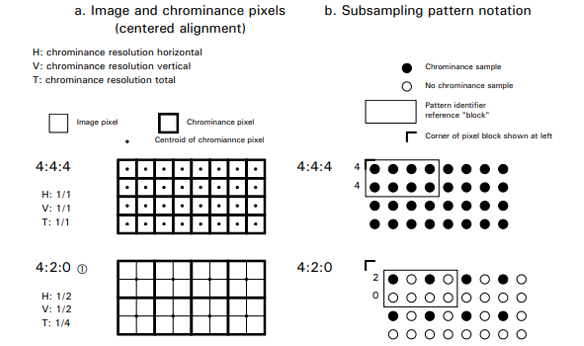
\includegraphics[width=\linewidth, center]{pics/chroma.png} 
\caption{Chrominance subsampling pattern for the 4:2:0 ratio.}
\label{fig:chroma}
\end{figure}

\paragraph{Block-based DCT}
After the color space conversion, the three components Y, $C_b$ and $C_r$ are partitioned into blocks of size 8x8. Each one of these blocks are then converted separately to a frequency-domain representation through a Discrete Cosine Transform (DCT).

The aim of the DCT is to redistribute the samples energy among a few transform coefficients, thus allowing a more efficient and compact representation of the information given by the image. This kind of transform is used instead of the DFT mainly for efficiency reasons.

The generic element $t_{kl}$ of the NxN 1-D Discrete Cosine Transformation matrix T is given by

\begin{equation}
t_{kl} = 
\begin{cases}
\sqrt{\frac{1}{N}} cos (\frac{\Pi}{2N}(k - 1)(2l - 1)), & k = 1 \\ 
\sqrt{\frac{2}{N}} cos (\frac{\Pi}{2N}(k - 1)(2l - 1)), & k = 2, 3 ... N
\end{cases}
\end{equation}
\begin{wrapfigure}{r}{0.4\textwidth}
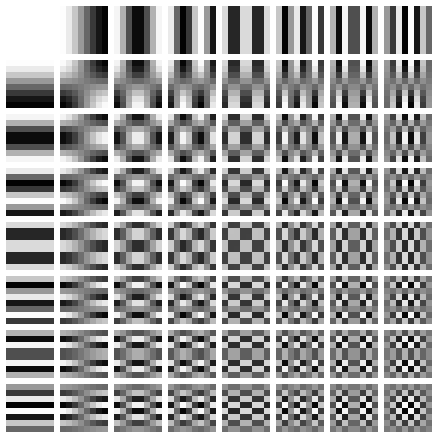
\includegraphics[width=0.95\linewidth, center]{pics/dct.png} 
\caption{Basis functions.}
\label{fig:dct}
\end{wrapfigure}

The 2-D version of the Dicrete Cosine Transform is applied to the image by running first a 1-D DCT along the rows, and then a 1-D DCT along the columns of the resulting matrix. 

Furthermore, the DCT can be regarded as a linear combination of the 64 patters, called basis functions, shown in Figure \ref{fig:dct}. An example of DCT output 8x8 matrix is given in (4). Notice that the coefficient in the top-left corner has much larger magnitude than the others; this particular coefficient is called DC and it represents the average color of the 8x8 region. The others are called AC coefficients.

\begin{equation}
\begin{bmatrix}
-303.59 & 47.62 & 104.27 & -53.12 &	-51.17 & 38.85 &	20.64 &	0.75 \\
-3.87 &	0.35 &	0.88 &	0.18 & -0.64 & 	-0.51 &	1.15 & 	8.87 \\
-0.24 &	-0.21 &	1.06 &	-1.60 &	1.14 & 	-0.08 &	-0.42 &	3.01 \\
0.24 &	-1.12 &	1.60 &	-1.12 &	-0.04 &	0.98 & 	-0.94 & 	-0.52 \\
0.52 &	0.16 &	-0.51 &	0.37 &	-0.13 &	0.06 &	-0.07 & 	1.25 \\
-2.04 &	1.19 &	0.35 &	-1.38 &	0.72 &	0.87 &	-1.32 &	0.32 \\
0.96 &	-0.08 &	-0.12 &	-0.28 &	0.42 &	-0.03 &	-0.23 &	0.10 \\
0.05 &	0.97 &	-1.28 &	0.57 & 0.37 &	-0.78 &	0.54 &	0.17
\end{bmatrix}
\end{equation}
Small valued coefficients define a rapid color change from one pixel to another within the 8x8 block (high frequency coefficients).

\paragraph{Quantization} The quantization step is the one that makes this type of image compression a lossy compression. The output matrix coefficients ,obtained by the DCT for every 8x8 block, are quantized, thus losing some information and making it impossible to recover the original values. 

The process takes advantage of two quantization tables suggested for the JPEG coding scheme: one for the luminance component (5a), and the other for the two chroma components (5b).

\begin{subequations}
\begin{tabularx}{\textwidth}{X X}
\begin{equation}
\begin{bmatrix}
16 &11 &10 &16&	24&	40&	51&	61\\
12&	12&	14&	19&	26&	58&	60&	55\\
14&	13&	16&	24&	40&	57&	69&	56\\
14&	17&	22&	29&	51&	87&	80&	62\\
18&	22&	37&	56&	68&	109&103&77\\
24&	35&	55&	64&	81	&104&113&92\\
49&	64&	78&	87&	103&121&120&101\\
72&	92&	95&	98&	112&100&103&99
\end{bmatrix}
\end{equation}
 &
\begin{equation}
\begin{bmatrix}
17&	18&	24&	47&	99&	99&	99&	99\\
18&	21&	26&	66&	99&	99&	99&	99\\
24&	26&	56&	99&	99&	99&	99&	99\\
47&	66&	99&	99&	99&	99&	99&	99\\
99&	99&	99&	99&	99&	99&	99&	99\\
99&	99&	99&	99&	99&	99&	99&	99\\
99&	99&	99&	99&	99&	99&	99&	99\\
99&	99&	99&	99&	99&	99&	99&	99
\end{bmatrix}
\end{equation}
\end{tabularx}
\end{subequations}

Notice that in both matricies the lower values are concentrated near the DC coefficient region (top-left corner). This is due to the fact that lower frequency coefficients are better perceived by the human eye, so they need a thinner quantization, whereas high frequency coefficients lose the most of their information.


The values of the quantization tables can be tuned in order to control the compression ratio of the image by means of a quality factor. This allows the JPEG scheme to adjust the quality of the compressed image and its size.

Formally, the quantized values are computed by rounding the output value from the DCT divided by the correspoding value of the quantization matrix:

\begin{equation}
F_{i, j} = \floor*{\frac{D_{i, j}}{Q_{i, j}} + 0.5}
\end{equation}

where D is the output matrix from the DCT for one of the three components and Q is the quantization matrix.\\

\paragraph{Huffman encoding}
In this step, the quantized values are coded using a zigzag ordered coding that starts from the DC coefficient and descend to the bottom as shown in Figure \ref{fig:zigzag}. 
In this way, the 8x8 block matrix is represented as a vector of length 64.

\begin{wrapfigure}{r}{0.4\textwidth}
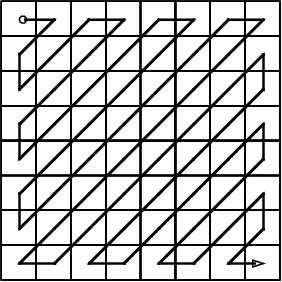
\includegraphics[width=0.95\linewidth, center]{pics/zigzag.png} 
\caption{Zigzag ordering.}
\label{fig:zigzag}
\end{wrapfigure}

The AC and DC coefficients are coded differently: the former ones are described by a pair defined as \{size, skip\} where size is the number of bits needed to represent the quantized frequency value, and skip is the number of zeros values that precedes it. This pair is then used as codeword for the Huffman coding procedure.

Instead, DC coefficients are coded using a sort of delta measure: each DC coefficient is compared to the previous one, and the difference is coded using Huffman coding.
\\

\subsection{MATLAB Implementation}
The first thing that the program does is to load the input image and check if any errors are present. Then, it extracts relevant informations such as the image dimension in kiloBytes and the number of rows and columns. In particular, a padding is applied if the image needs to reach a desired size (in this case we need to perform a 8x8 block division, so we need the number of rows and columns to be multiples of 8).

The color space conversion is exploited through the MATLAB function \texttt{rgb2ycbcr} and then the components are centered to 0. Also, chroma subsampling is applied by downsampling the $C_b$ and $C_r$ matricies.

After that, the 2-D Discrete Cosine Transform is applied to each component by means of the function \texttt{dct2} exploited through \texttt{blockproc}, so that it works separately in each different 8x8 block.

At this point, a quality factor needs to be set in order to obtain the proper quantization tables. The value is selected between 0 and 100 (in percentage) and each coefficient of the quantization table is recomputed as:

\begin{equation}
Q_{i, j}' = Q_{i, j} \cdot \frac{1}{q_{f}} \cdot 50
\end{equation}

where $q_{f}$ is the quality factor. In this way $Q_{i, j}' = Q_{i, j}$ whenever the quality factor is 50\% as specified in the standard JPEG coding scheme.

The quantization tables are then used in order to quantize the DCT coefficients according to the equation (6) seen in the previous section. Also in this case the function \texttt{blocproc} has been used to work on separate 8x8 blocks.

Finally, the encoding has been computed using the MATLAB function \texttt{huffmanenco} which requires in input the quantized DCT coefficients and the dictionary that describes it. The dictionary has been computed by calling the function \texttt{huffmandict} which requires as input the symbols and their probability, the former being the unique occurencies of the quantized DCT coefficients and the latter being the ratio between the number of that particular symbol occurencies and the total number of occurencies. 

To decode and reconstruct the image, all the previous steps have been processed backwards, again using \texttt{blocproc} for 8x8 block processing and \texttt{huffmandeco} to decode the codewords generated by \texttt{huffmanenco}.

\section{Results}
To evaluate the performances of the algorithm with respect to different images and different quality factors, the following parameters have been computed:

\begin{itemize}
  \item The \texttt{size of the encoded image} is found as the size of the encoded Y, $C_b$ and $C_r$ arrays and it is expressed in kB.
  \item The \texttt{compression ratio} is the original image size divided by the encoded image size.
  \item The \texttt{computational complexity} is expressed in seconds and tells how much it took to perform the compression.
  \item The \texttt{bpp} parameter is the size of the compressed image in bits divided by the total number of pixels.
  \item Finally, the \texttt{PSNR} (Peak Signal to Noise Ratio) is the ratio between the maximum possible power of the image signal and the noise. It is measured in dB and can be defined as:
  
\begin{equation}
PSNR = 10 log_{10} \frac{255^{2}}{MSE}
\end{equation}

where the MSE (Mean Squared Error) for an image of size MxN is computed as:

\begin{equation}
MSE = \frac{\sum\limits_{M, N} [I_{original}(m, n) - I_{compressed}(m, n)]^{2}}{M N}
\end{equation}
\end{itemize}

Five images (taken from the Kodak image dataset) were tested with different quality factors. By increasing the amount of compression the results obtained show more and more visible artifacts with respect to the original images as Figure \ref{fig:qualities} shows.

\begin{figure}[h]
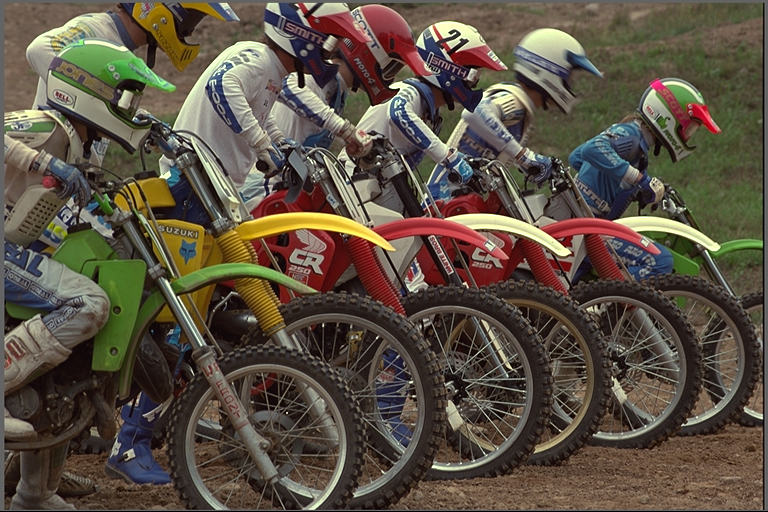
\includegraphics[width=0.8\linewidth, center]{dataset/kodim05.png} 
\caption{Sample image.}
\label{fig:moto}
\end{figure}

\begin{figure}[ht!]
     \begin{center}
%
        \subfigure[Quality factor = 5]{%
            \label{fig:first}
            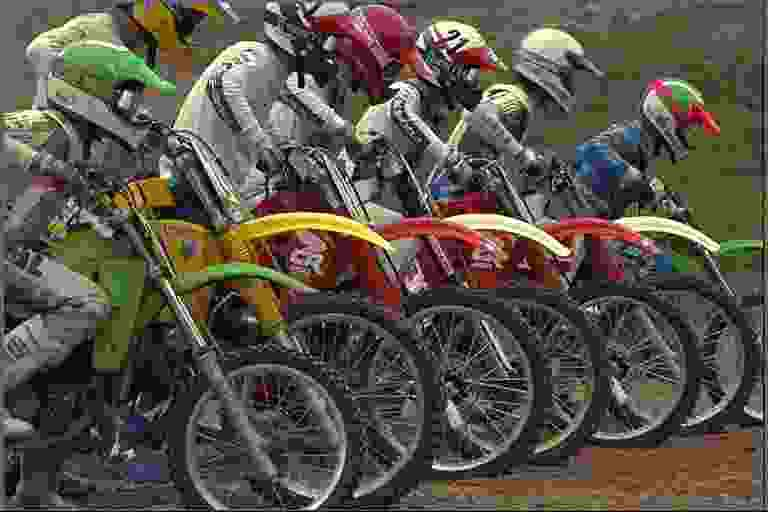
\includegraphics[width=0.22\textwidth]{out/05q5.jpeg}
        }%
        \subfigure[Quality factor = 15]{%
           \label{fig:second}
           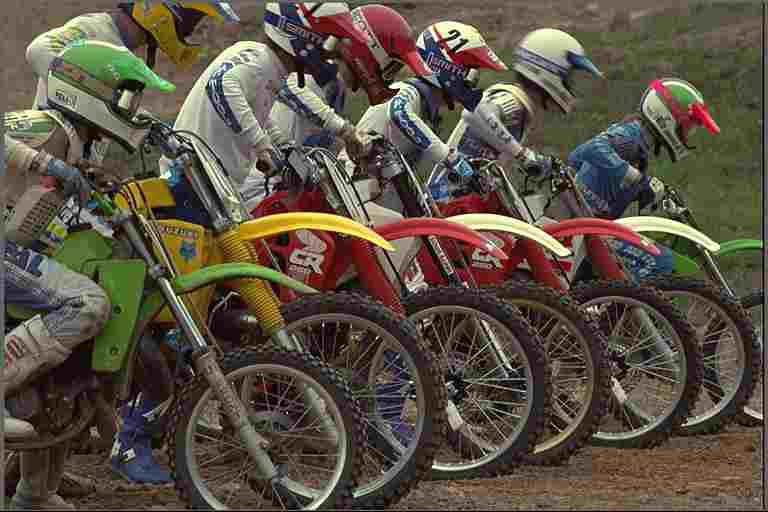
\includegraphics[width=0.22\textwidth]{out/05q15.jpeg}
        }%
        \subfigure[Quality factor = 30]{%
            \label{fig:first}
            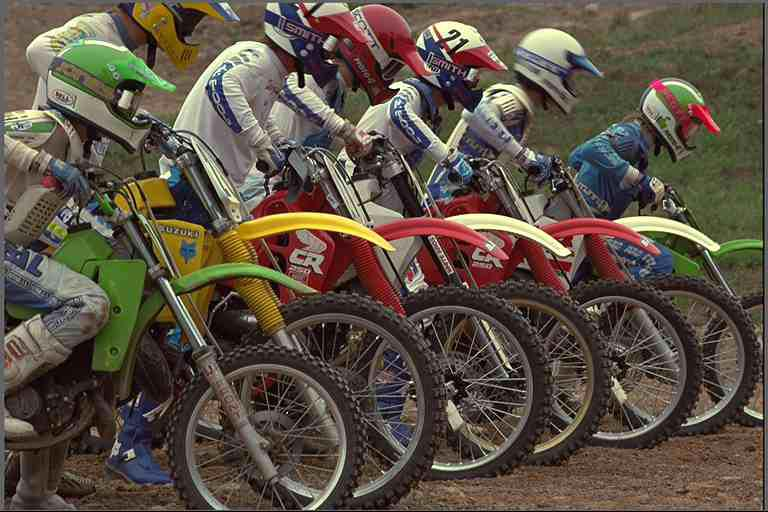
\includegraphics[width=0.22\textwidth]{out/05q30.jpeg}
        }%
        \subfigure[Quality factor = 50]{%
            \label{fig:third}
            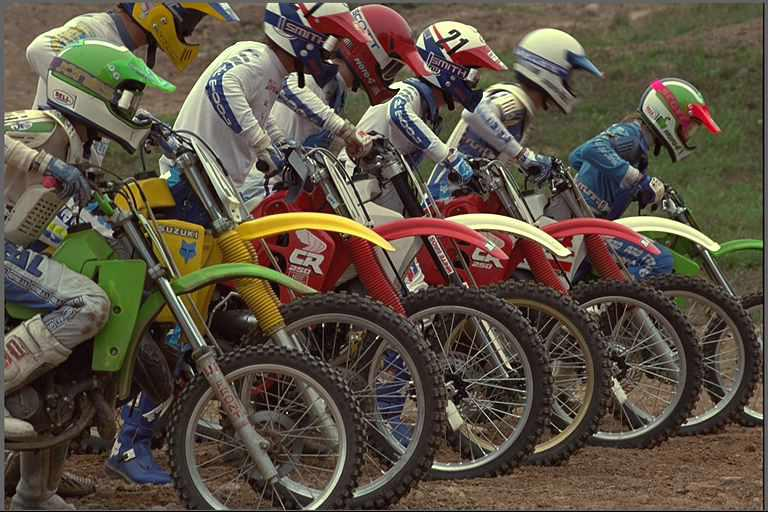
\includegraphics[width=0.22\textwidth]{out/05q50.jpeg}
        }\\
        \subfigure[Quality factor = 65]{%
            \label{fig:fourth}
            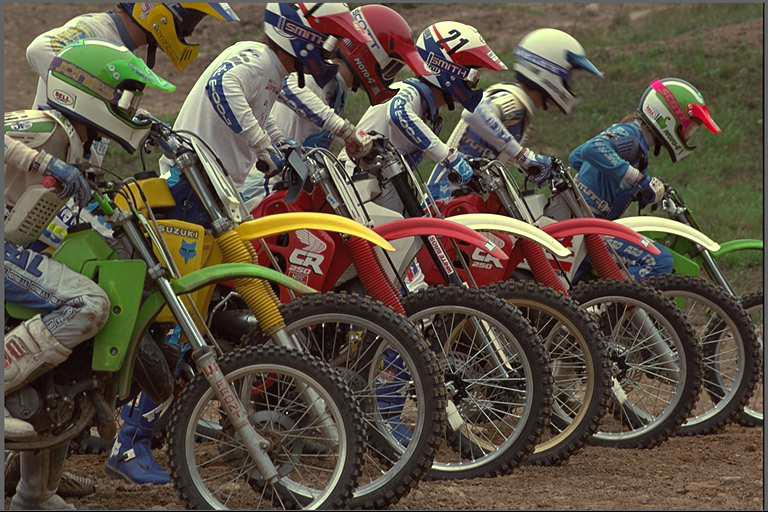
\includegraphics[width=0.3\textwidth]{out/05q65.jpeg}
        }%
        \subfigure[Quality factor = 80]{%
            \label{fig:third}
            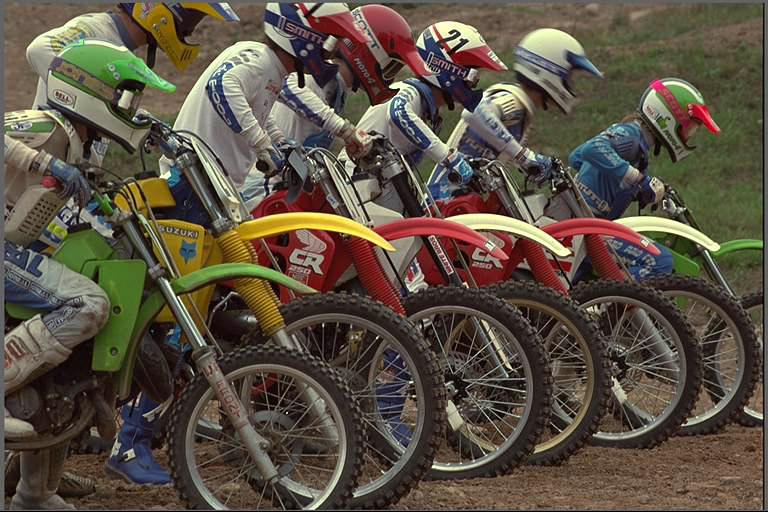
\includegraphics[width=0.3\textwidth]{out/05q80.jpeg}
        }%
        \subfigure[Quality factor = 100]{%
            \label{fig:fourth}
            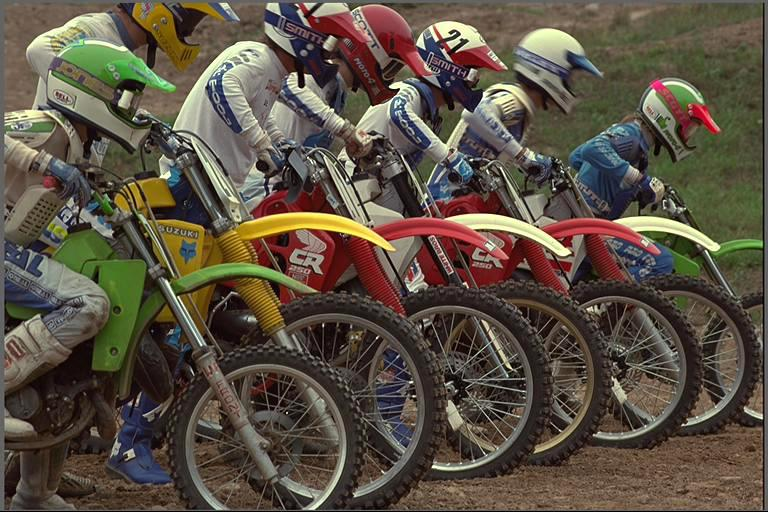
\includegraphics[width=0.3\textwidth]{out/05q100.jpeg}
        }%
%
    \end{center}
    \vspace*{-7mm}
    \caption{Compression with different quality values.}
\label{fig:qualities}
\end{figure}

\begin{center}
\begin{table}[h!]
  \centering
\begin{tabular}{ |c|c|c|c|c|c|c| } 
\hline
Image & Quality & Enc. Size [kB] & C. Ratio & Time [s] & bpp & PSNR [dB] \\
\hline
\multirow{3}{4.2em}{Motocross\\ (Original Size:\\1179.64 kB)} 
& 5 & 78.55 & 15.01 & 3.40 & 1.59 & 20.75\\ 
& 15 & 89.76 & 13.14 & 3.66 & 1.83 & 24.70\\ 
& 30 & 103.13 & 11.44 & 4.18 & 2.10 & 27.01 \\ 
& 50 & 117.14 & 10.07 & 4.63 & 2.38 & 28.75 \\ 
& 65 & 126.18 & 9.35 & 5.21 & 2.57 & 29.70 \\
& 80 & 133.44 & 8.84 & 5.45 & 2.71 & 30.42 \\
& 100 & 142.56 & 8.27 & 6.18 & 2.90 & 31.19 \\
\hline
\end{tabular}
\vspace*{-2mm}
\caption{Parameters found for different quality levels.}
\label{table:quality}
\end{table}
\end{center}

\vspace{-10mm}

Notice in Table \ref{table:quality} how the parameters change according to the quality factor: the size, computational time and bpp values increase almost linearly, while the compression ratio and PSNR parameters follow a particular shape shown in Figure \ref{fig:plots}. Both these parameters are the ones that change the most with respect to the other ones over the different quality factors.

\begin{figure}[ht!]
     \begin{center}
%
        \subfigure{%
            \label{fig:first}
            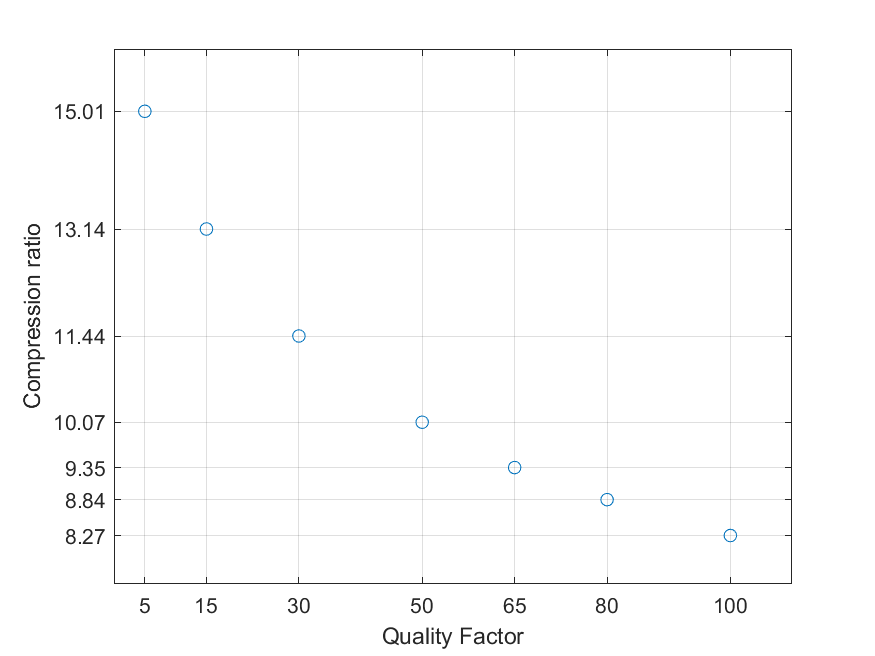
\includegraphics[width=0.5\textwidth]{ratio.png}
        }%
        \subfigure{%
           \label{fig:second}
           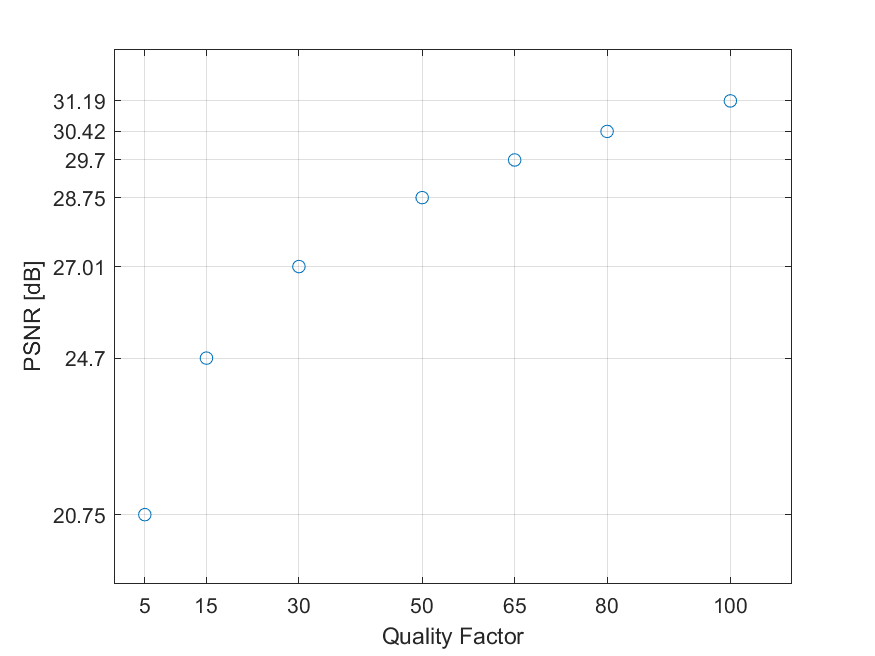
\includegraphics[width=0.5\textwidth]{psnr.png}
        }
    \end{center}
    \caption{Plots of the compression ratio and PSNR parameters trends.}
    \label{fig:plots}
\end{figure}

Figure \ref{fig:chromacomp} shows a comparison between the algorithm applied with and without expoliting the chroma subsampling technique. Both images were compressed with a quality factor of 50. It is difficult to visually identify any significant difference between the two; however, as shown in Table \ref{table:chromacomp}, the chroma subsampling approach performs much better in terms of both time and size of the output image.

\begin{figure}[ht!]
     \begin{center}
%
        \subfigure[With chroma subsampling]{%
            \label{fig:first}
            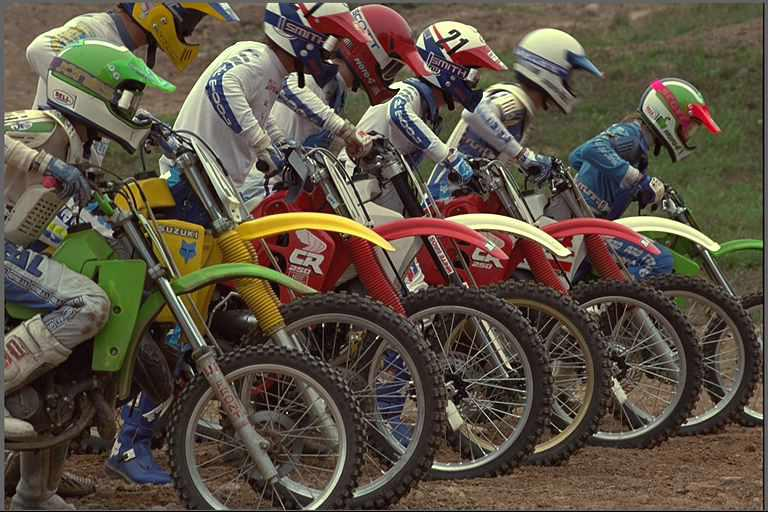
\includegraphics[width=0.5\textwidth]{out/05q50.jpeg}
        }%
        \subfigure[Without chroma subsampling]{%
           \label{fig:second}
           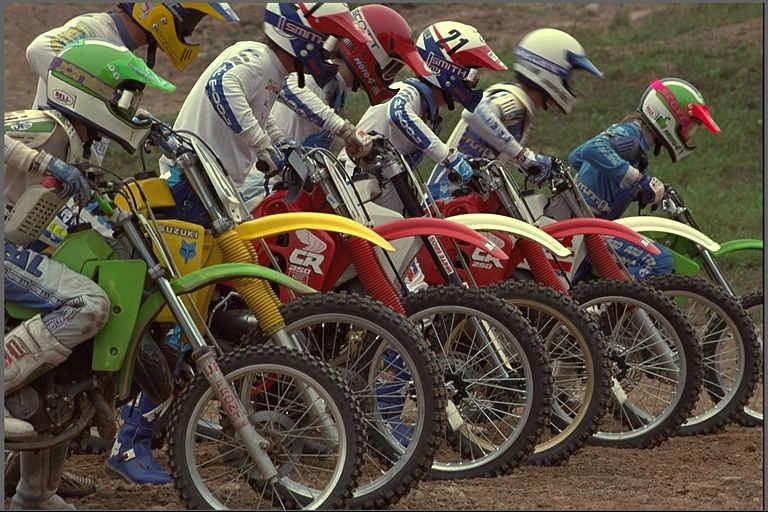
\includegraphics[width=0.5\textwidth]{out/chroma.jpeg}
        }
    \end{center}
    \caption{Chroma subsampling comparison.}
    \label{fig:chromacomp}
\end{figure}

\begin{center}
\begin{table}[h!]
  \centering
\begin{tabular}{ |c|c|c|c|c|c| } 
\hline
Chroma Sub. & Enc. Size [kB] & C. Ratio & Time [s] & bpp & PSNR [dB] \\
\hline
Yes & 117.14 & 10.07 & 4.63 & 2.38 & 28.75 \\ 
No & 197.37 & 5.97 & 12.26 & 4.01 & 29.52 \\
\hline
\end{tabular}
\caption{Chroma subsampling comparison table.}
\label{table:chromacomp}
\end{table}
\end{center}

\subsection{Comparison with the JPEG standard}
The default MATLAB implementation of the JPEG standard has been exploited using \texttt{imwrite} and tuning the quality of the output image. Figure \ref{fig:jpegcomp} shows a comparison between the results of the two coding schemes with a quality factor of 5: the two algorithms give similar results but in many parts of the image it is possible to notice that the colors are clustered in a different way. In the zoomed part reported in the top right corner, the area covered by the dark green color is much more present in the JPEG standard from MATLAB than in my implementation. This is probably due to the way the data has been quantized and, in particular, it depends on the choice of the rounding operation done for the quantization table (Equation (6)).

\begin{figure}[ht!]
     \begin{center}
%
        \subfigure[JPEG-like compression]{%
            \label{fig:first}
            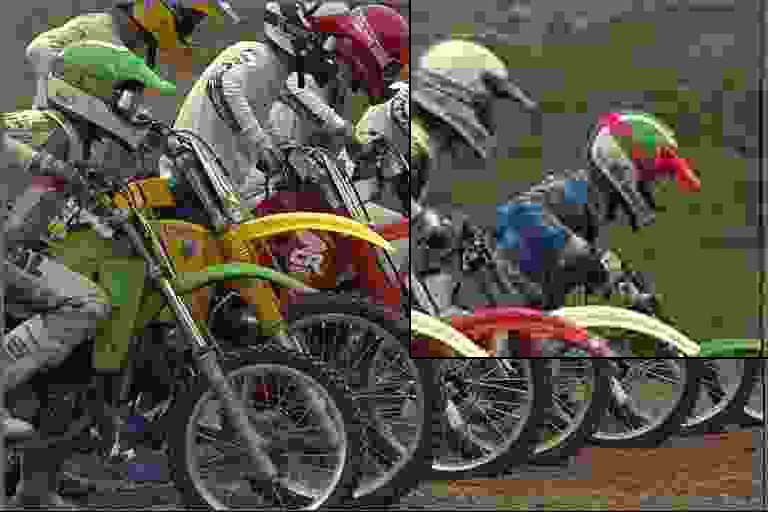
\includegraphics[width=0.5\textwidth]{out5comp.png}
        }%
        \subfigure[Standard JPEG compression]{%
           \label{fig:second}
           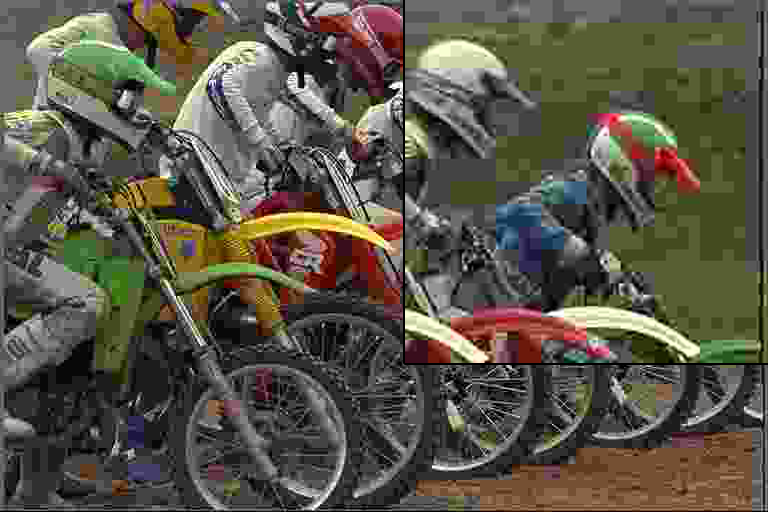
\includegraphics[width=0.5\textwidth]{jpeg5comp.png}
        }
    \end{center}
    \caption{Comparison with the standard JPEG implementation.}
    \label{fig:jpegcomp}
\end{figure}

In Table \ref{table:jpegcomp} are reported some relevant features extracted from the JPEG implementation present in MATLAB. The standard coding scheme clearly gives better results in terms of size of the output image and most of all in terms of computational time. The PSNR, instead, gives similar results, as Figure \ref{fig:psnrcomp} shows. The curve follows the same shape as the one seen for my implementation and the values are slightly higher for the standard algorithm: the difference becomes more and more visible for higher quality factors, whereas for higher compression this difference is not significant. In particular, notice that the PSNR of the standard JPEG algorithm for a quality factor of 65 is even higher than the PSNR of my program for a quality factor of 80.

\begin{center}
\begin{table}[h!]
  \centering
\begin{tabular}{ |c|c|c|c|c|c|c| } 
\hline
Approach & Quality & Enc. Size [kB] & Time [s] & PSNR [dB] \\
\hline
\multirow{3}{4.2em}{Standard JPEG} 
& 5 & 14.9 & 0.02 & 21.41 \\ 
& 15 & 31.8 & 0.04 & 25.36\\ 
& 30 & 49.7 & 0.04 & 27.73 \\ 
& 50 & 67.4 & 0.04 & 29.59  \\ 
& 65 & 82.7 & 0.06 & 30.96 \\
& 80 & 112 & 0.06 & 33.30\\
\hline
\multirow{3}{4.2em}{JPEG-like}
& 5 & 78.55 & 3.40 & 20.75\\ 
& 15 & 89.76 & 3.66 & 24.70\\ 
& 30 & 103.13 &  4.18 & 27.01 \\ 
& 50 & 117.14 & 4.63 & 28.75 \\ 
& 65 & 126.18 & 5.21 & 29.70 \\
& 80 & 133.44 &  5.45 & 30.42 \\
\hline
\end{tabular}
\caption{Comparison with the Standard JPEG implementation table.}
\label{table:jpegcomp}
\end{table}
\end{center}
\vspace{-10mm}


\begin{figure}[H]
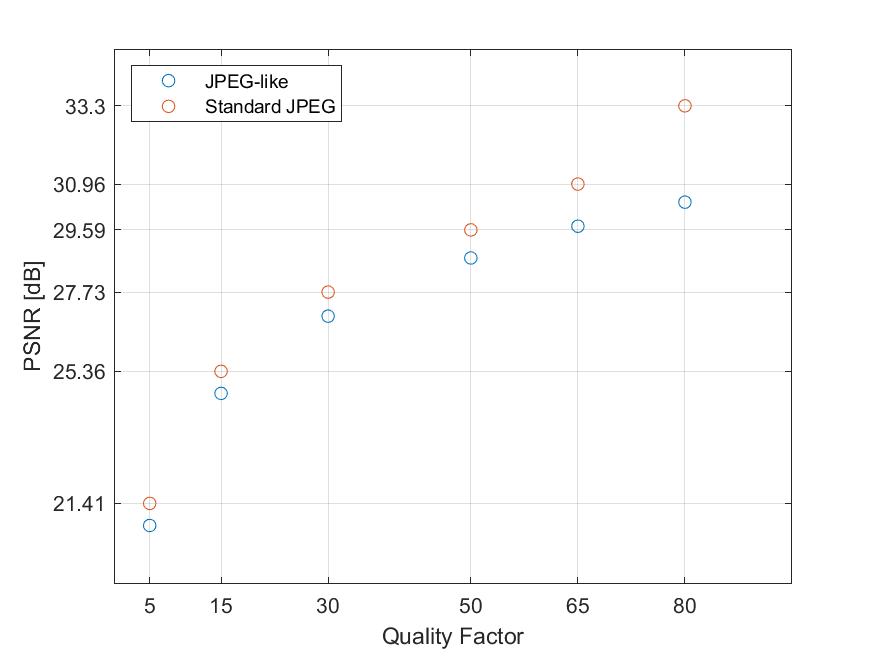
\includegraphics[width=0.7\linewidth, center]{jpegcomp.png} 
\caption{PSNR comparison.}
\label{fig:psnrcomp}
\end{figure}


In the following pages I will report some visual comparison between the two approaches and also the outputs of my algorithm for the other images that were tested.


\begin{figure}[H]
     \begin{center}
%
		\subfigure[Quality = 15 (JPEG-like)]{%
            \label{fig:first}
            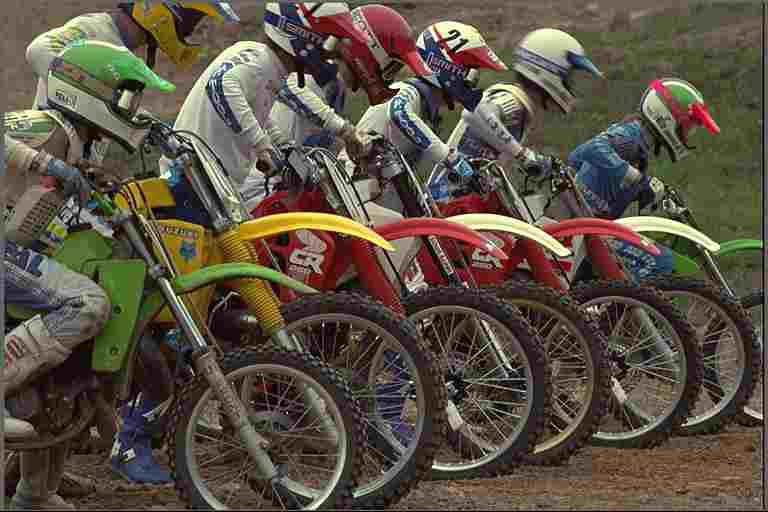
\includegraphics[width=0.4\textwidth]{out/05q15.jpeg}
        }%
        \subfigure[Quality = 15 (Standard JPEG)]{%
            \label{fig:first}
            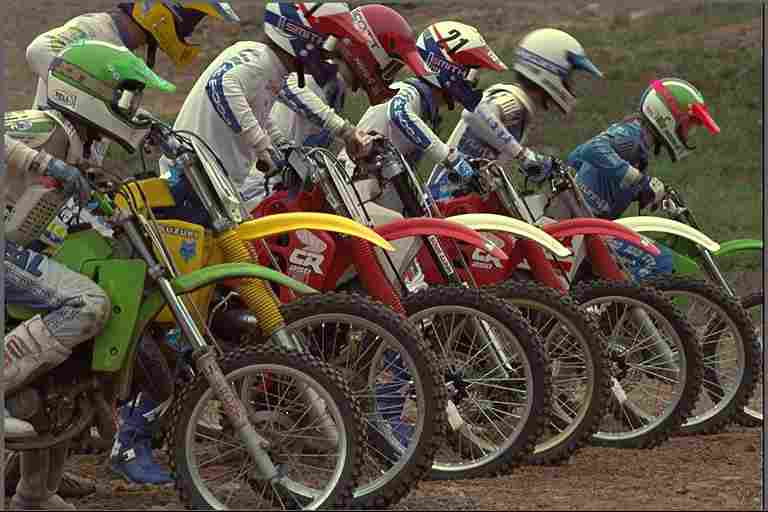
\includegraphics[width=0.4\textwidth]{jpeg/05q15.jpeg}
        }\\
        \subfigure[Quality = 30 (JPEG-like)]{%
           \label{fig:second}
           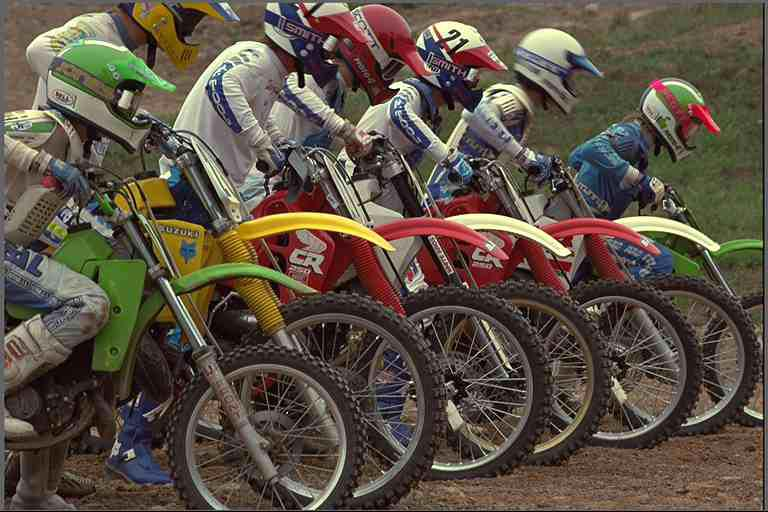
\includegraphics[width=0.4\textwidth]{out/05q30.jpeg}
        }%
        \subfigure[Quality = 30 (Standard JPEG)]{%
            \label{fig:first}
            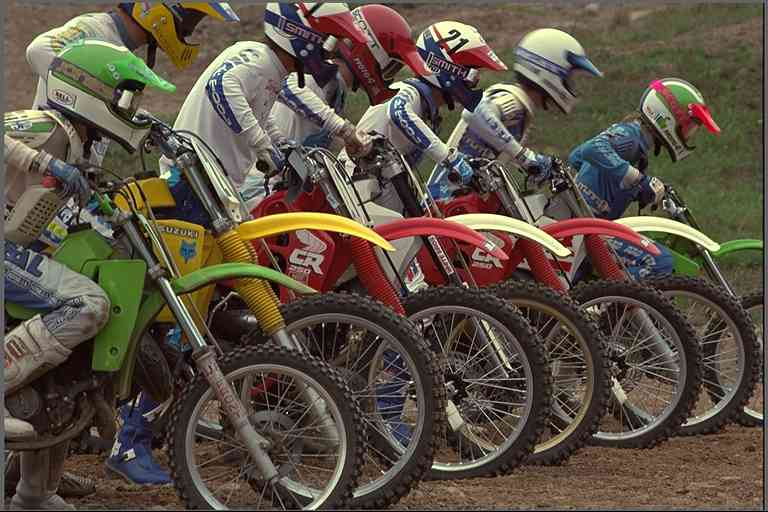
\includegraphics[width=0.4\textwidth]{jpeg/05q30.jpeg}
        }\\
        \subfigure[Quality = 50 (JPEG-like)]{%
            \label{fig:third}
            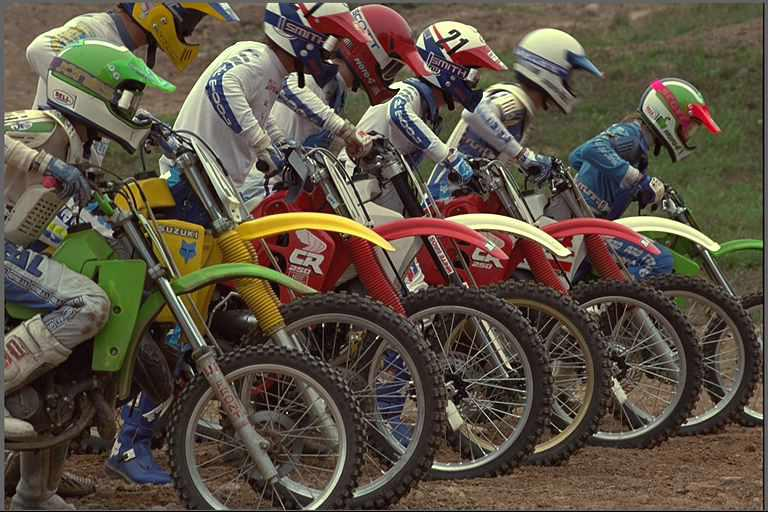
\includegraphics[width=0.4\textwidth]{out/05q50.jpeg}
        }%
        \subfigure[Quality = 50 (Standard JPEG)]{%
            \label{fig:fourth}
            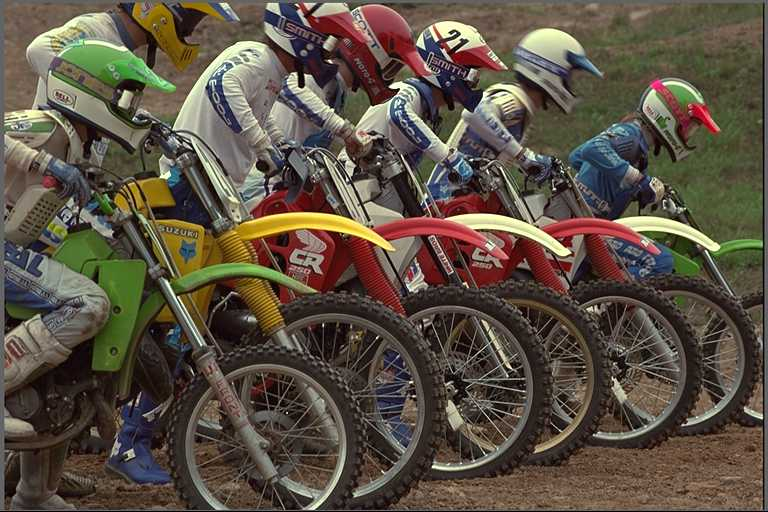
\includegraphics[width=0.4\textwidth]{jpeg/05q50.jpeg}
        }\\
        \subfigure[Quality = 80 (JPEG-like)]{%
            \label{fig:third}
            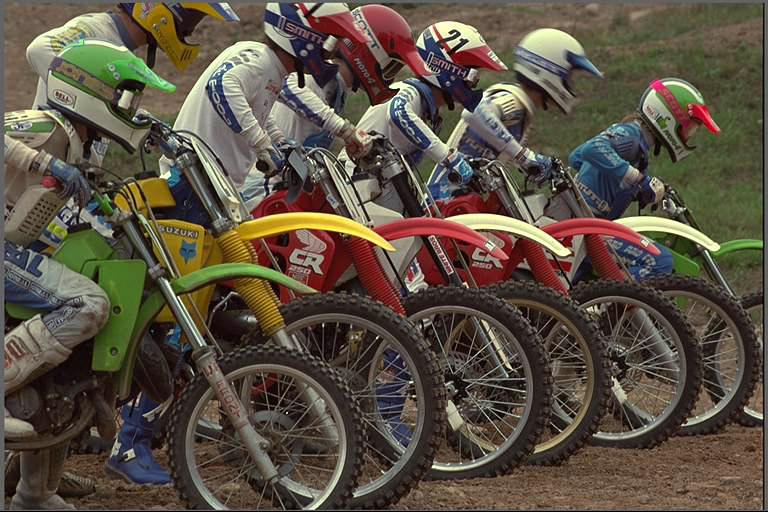
\includegraphics[width=0.4\textwidth]{out/05q80.jpeg}
        }%
        \subfigure[Quality = 80 (Standard JPEG)]{%
            \label{fig:fourth}
            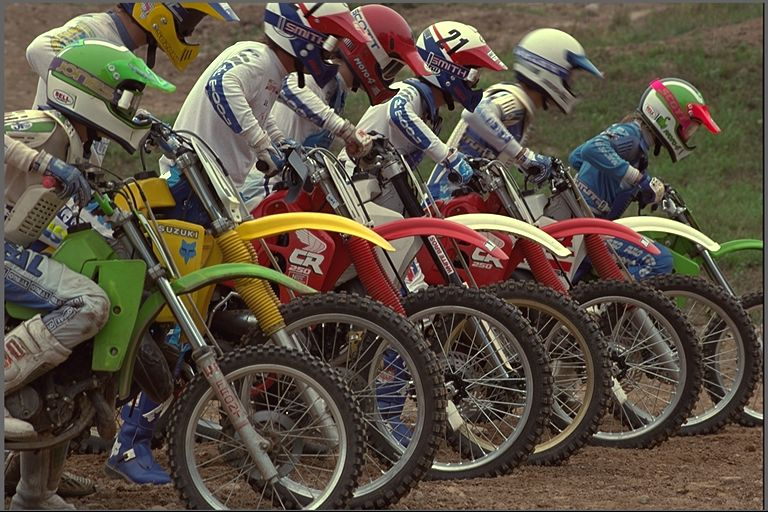
\includegraphics[width=0.4\textwidth]{jpeg/05q80.jpeg}
        }%
%
    \end{center}
    \caption{Comparison between the two approaches.}
\end{figure}


\begin{figure}[H]
     \begin{center}
%
		\subfigure[Original]{%
            \label{fig:first}
            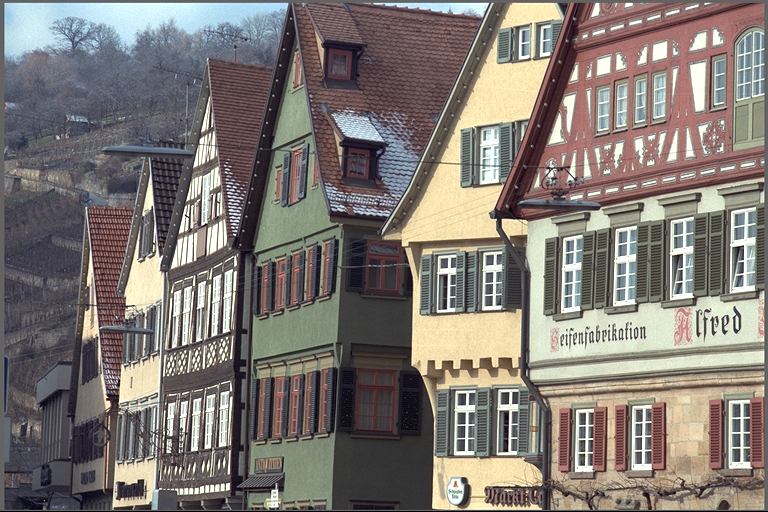
\includegraphics[width=0.4\textwidth]{dataset/kodim08.png}
        }%
        \subfigure[Quality factor = 5]{%
            \label{fig:first}
            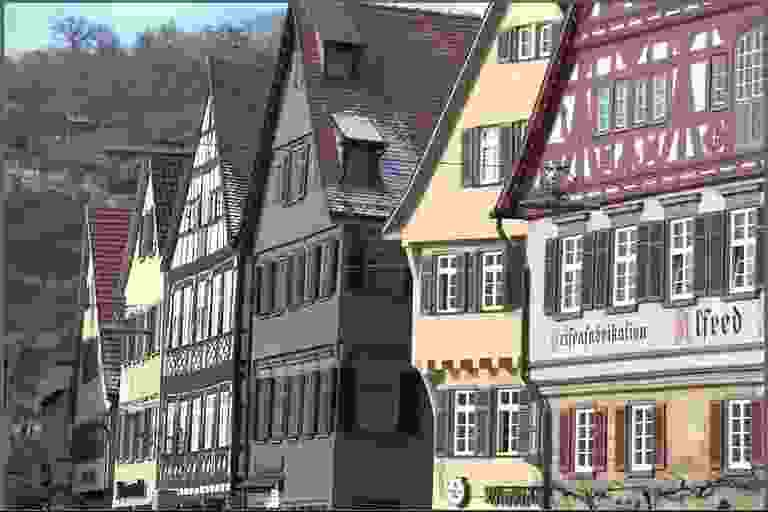
\includegraphics[width=0.4\textwidth]{out/08q5.jpeg}
        }\\
        \subfigure[Quality factor = 15]{%
           \label{fig:second}
           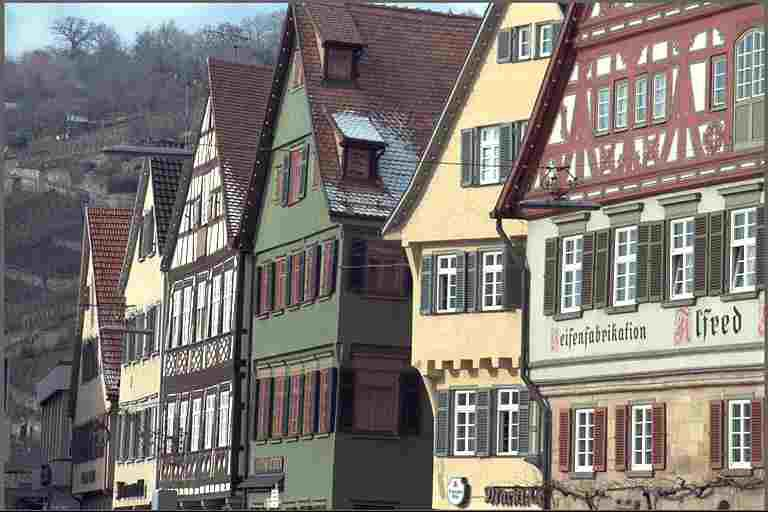
\includegraphics[width=0.4\textwidth]{out/08q15.jpeg}
        }%
        \subfigure[Quality factor = 30]{%
            \label{fig:first}
            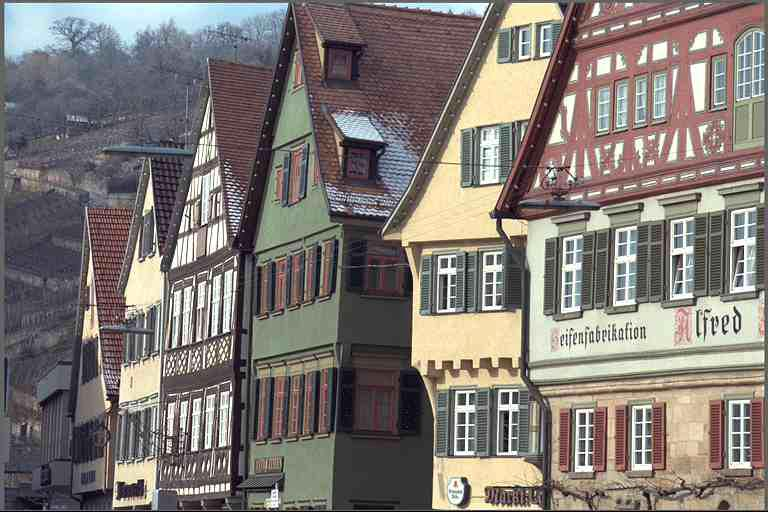
\includegraphics[width=0.4\textwidth]{out/08q30.jpeg}
        }\\
        \subfigure[Quality factor = 50]{%
            \label{fig:third}
            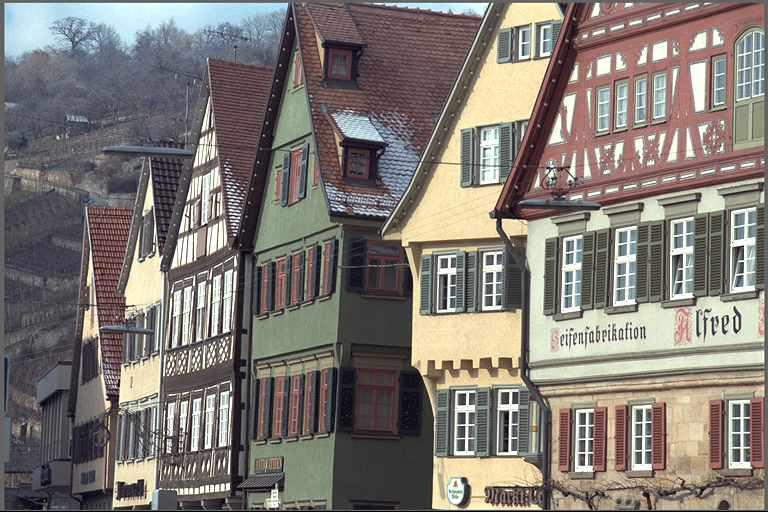
\includegraphics[width=0.4\textwidth]{out/08q50.jpeg}
        }%
        \subfigure[Quality factor = 65]{%
            \label{fig:fourth}
            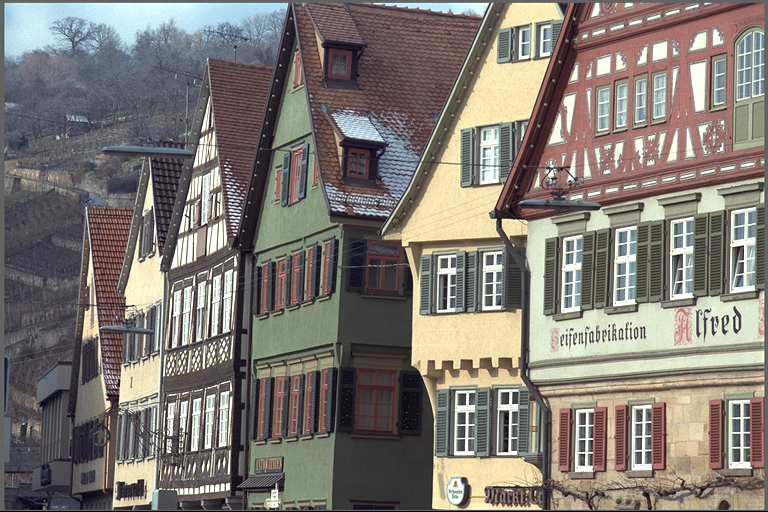
\includegraphics[width=0.4\textwidth]{out/08q65.jpeg}
        }\\
        \subfigure[Quality factor = 80]{%
            \label{fig:third}
            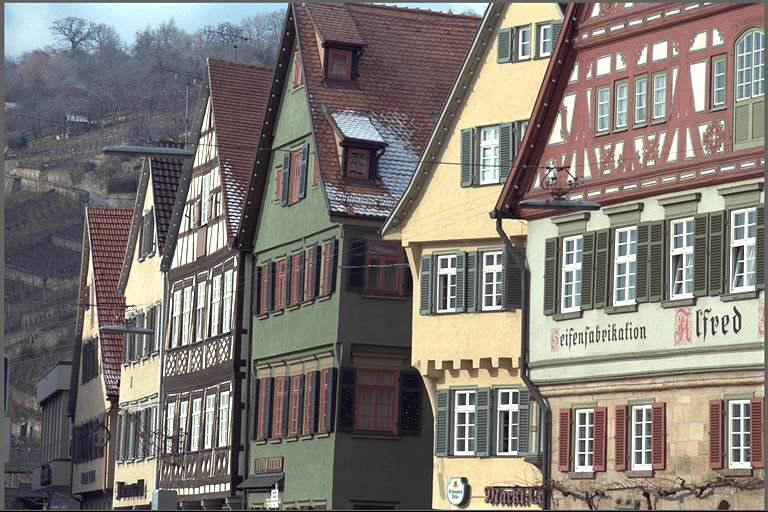
\includegraphics[width=0.4\textwidth]{out/08q80.jpeg}
        }%
        \subfigure[Quality factor = 100]{%
            \label{fig:fourth}
            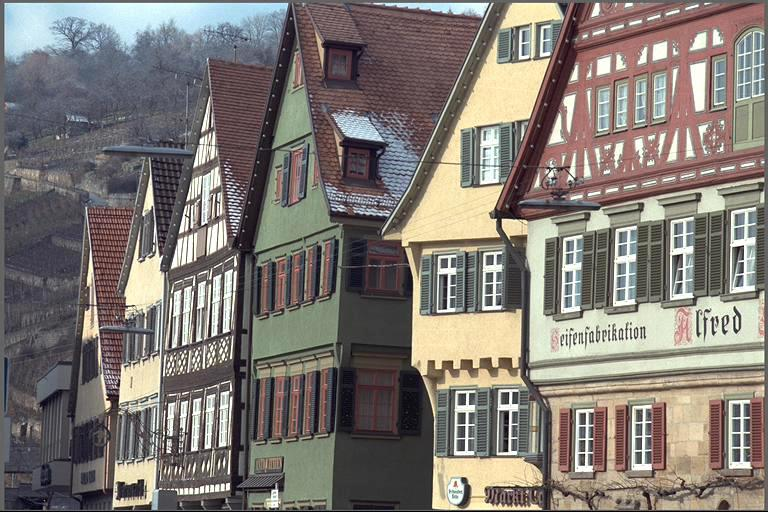
\includegraphics[width=0.4\textwidth]{out/08q100.jpeg}
        }%
%
    \end{center}
    \caption{kodim08.png}
\end{figure}

\begin{figure}[H]
     \begin{center}
%
		\subfigure[Original]{%
            \label{fig:first}
            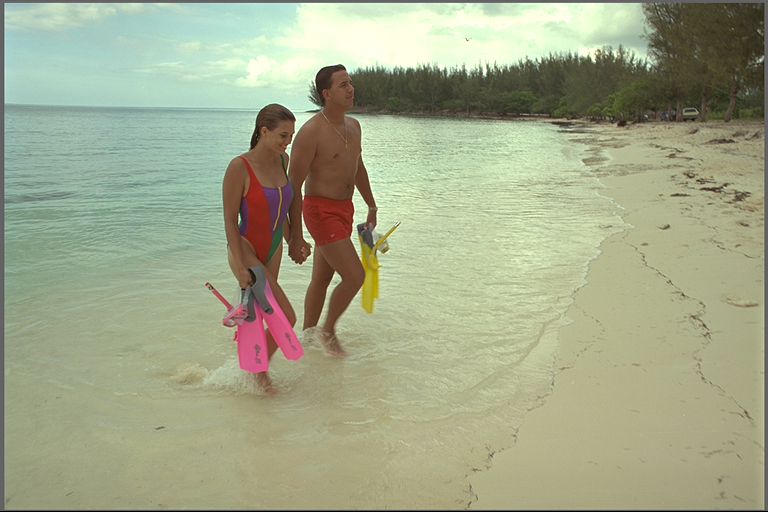
\includegraphics[width=0.4\textwidth]{dataset/kodim12.png}
        }%
        \subfigure[Quality factor = 5]{%
            \label{fig:first}
            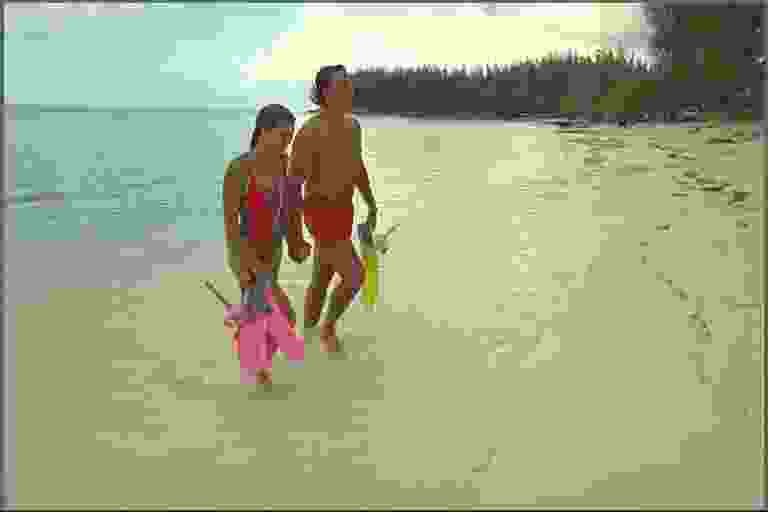
\includegraphics[width=0.4\textwidth]{out/12q5.jpeg}
        }\\
        \subfigure[Quality factor = 15]{%
           \label{fig:second}
           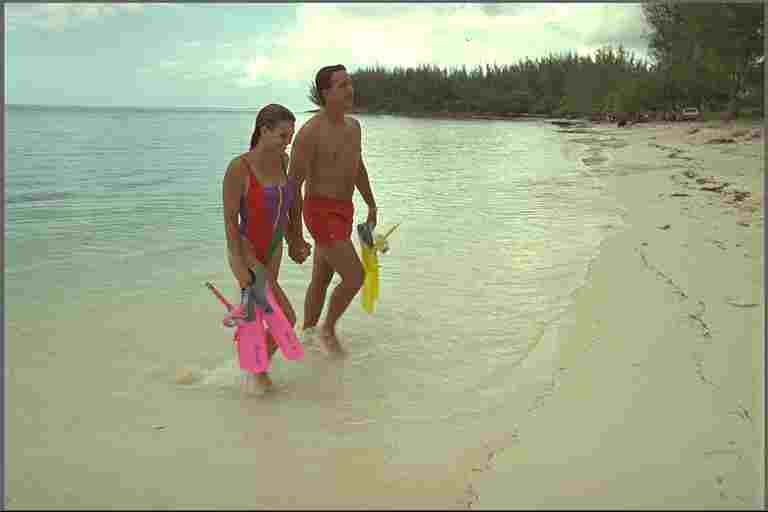
\includegraphics[width=0.4\textwidth]{out/12q15.jpeg}
        }%
        \subfigure[Quality factor = 30]{%
            \label{fig:first}
            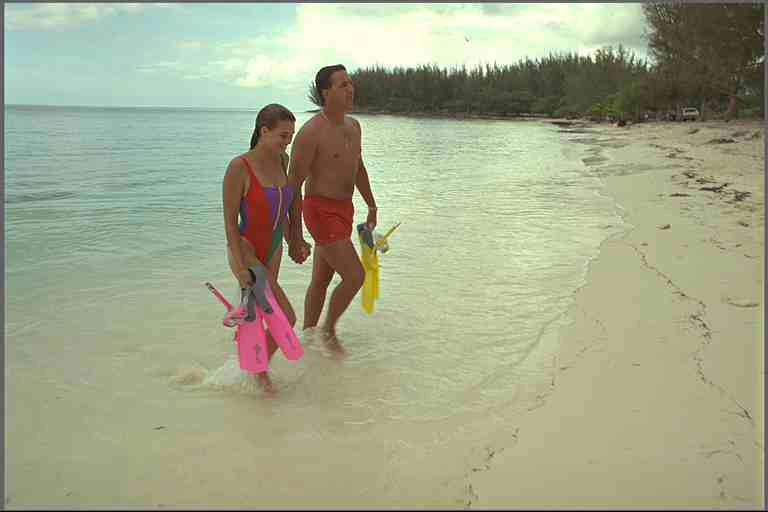
\includegraphics[width=0.4\textwidth]{out/12q30.jpeg}
        }\\
        \subfigure[Quality factor = 50]{%
            \label{fig:third}
            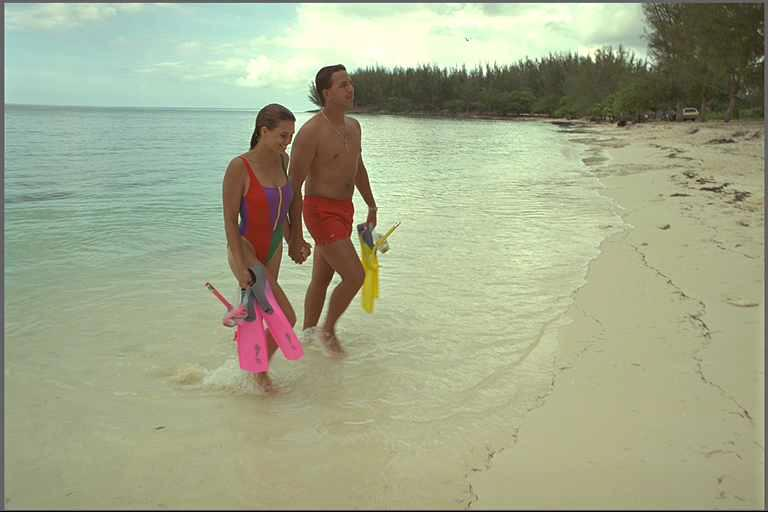
\includegraphics[width=0.4\textwidth]{out/12q50.jpeg}
        }%
        \subfigure[Quality factor = 65]{%
            \label{fig:fourth}
            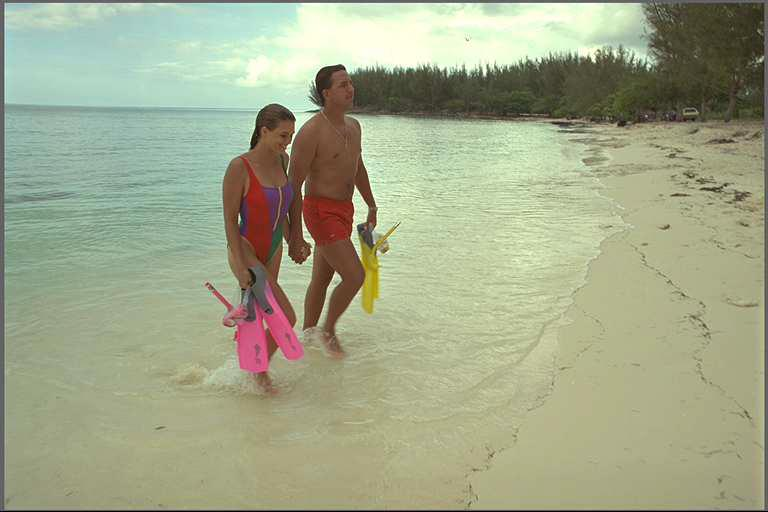
\includegraphics[width=0.4\textwidth]{out/12q65.jpeg}
        }\\
        \subfigure[Quality factor = 80]{%
            \label{fig:third}
            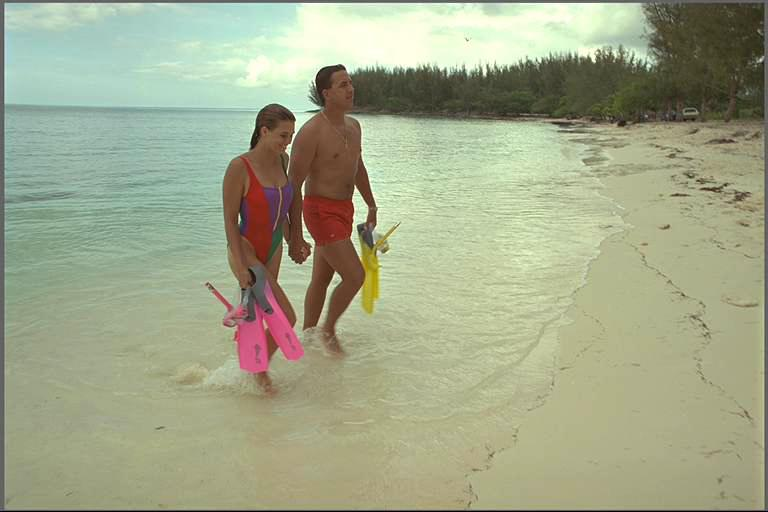
\includegraphics[width=0.4\textwidth]{out/12q80.jpeg}
        }%
        \subfigure[Quality factor = 100]{%
            \label{fig:fourth}
            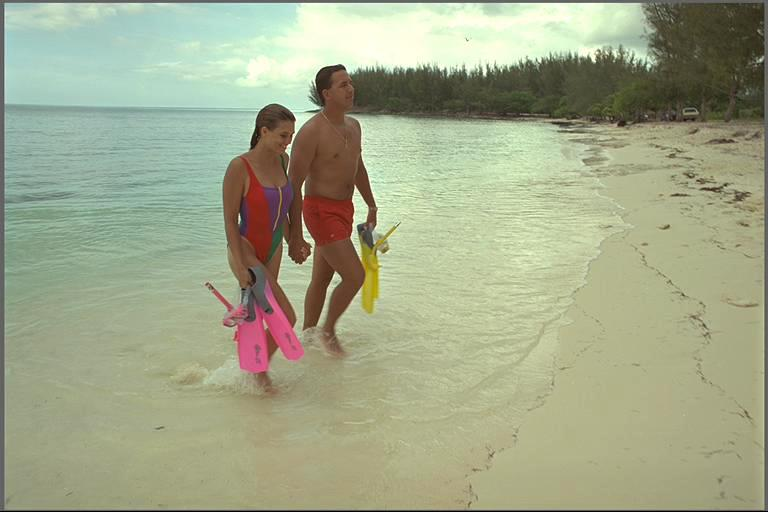
\includegraphics[width=0.4\textwidth]{out/12q100.jpeg}
        }%
%
    \end{center}
    \caption{kodim12.png}
\end{figure}

\begin{figure}[H]
     \begin{center}
%
		\subfigure[Original]{%
            \label{fig:first}
            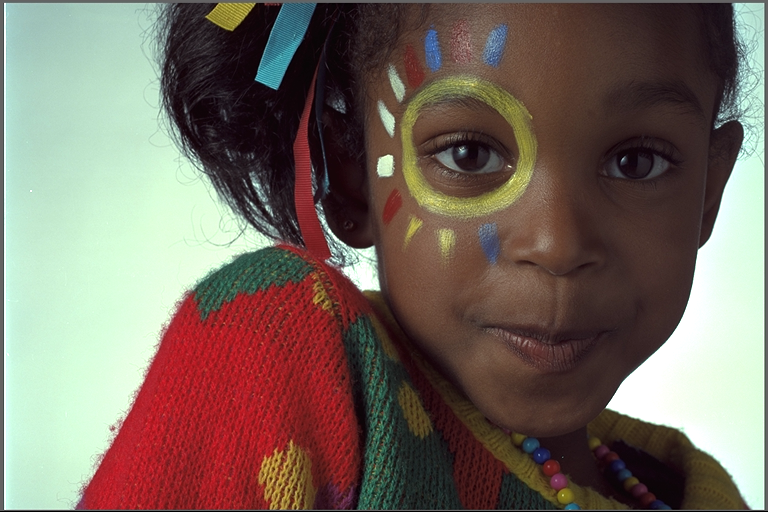
\includegraphics[width=0.4\textwidth]{dataset/kodim15.png}
        }%
        \subfigure[Quality factor = 5]{%
            \label{fig:first}
            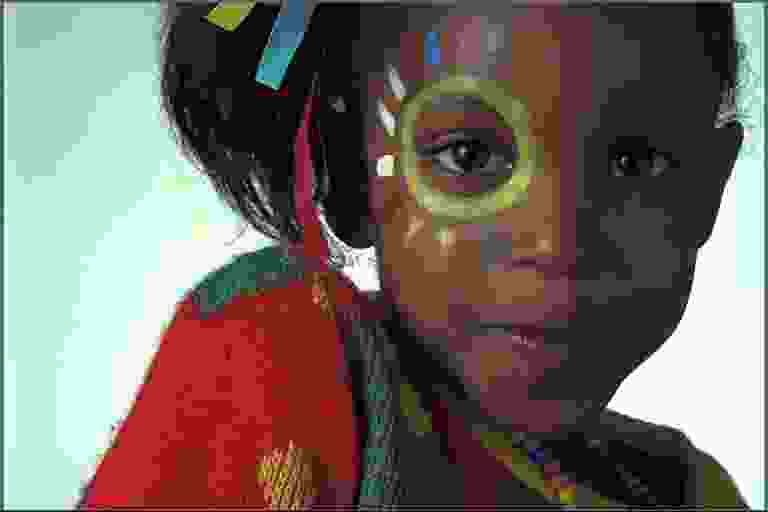
\includegraphics[width=0.4\textwidth]{out/15q5.jpeg}
        }\\
        \subfigure[Quality factor = 15]{%
           \label{fig:second}
           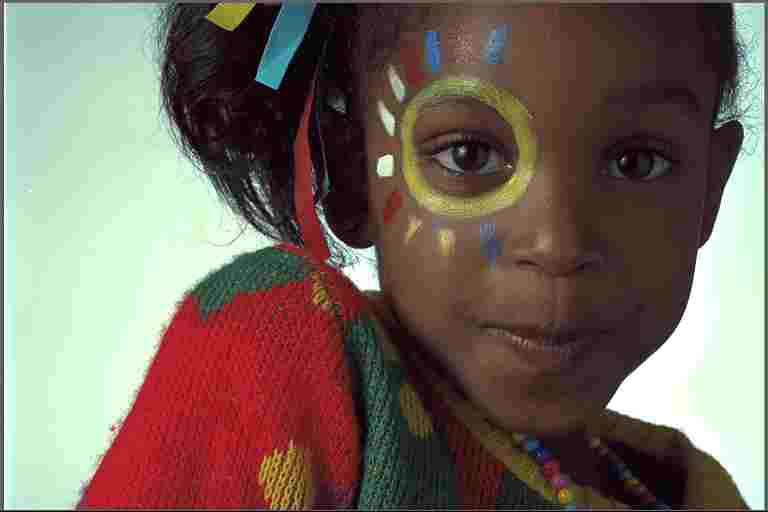
\includegraphics[width=0.4\textwidth]{out/15q15.jpeg}
        }%
        \subfigure[Quality factor = 30]{%
            \label{fig:first}
            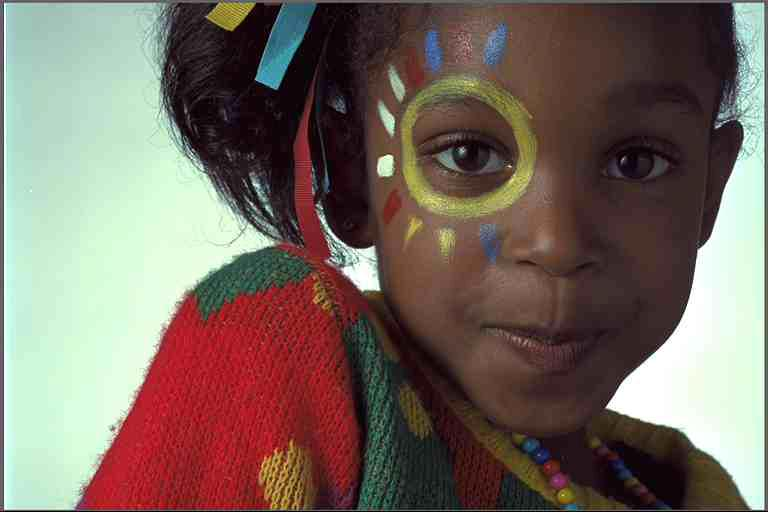
\includegraphics[width=0.4\textwidth]{out/15q30.jpeg}
        }\\
        \subfigure[Quality factor = 50]{%
            \label{fig:third}
            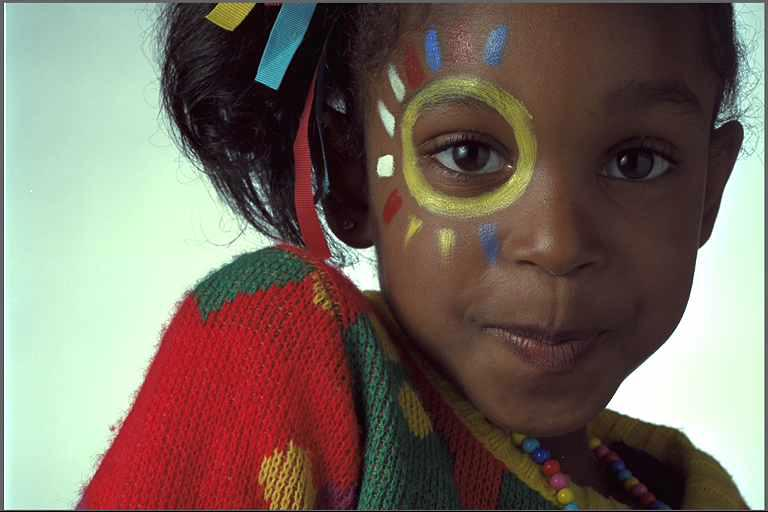
\includegraphics[width=0.4\textwidth]{out/15q50.jpeg}
        }%
        \subfigure[Quality factor = 65]{%
            \label{fig:fourth}
            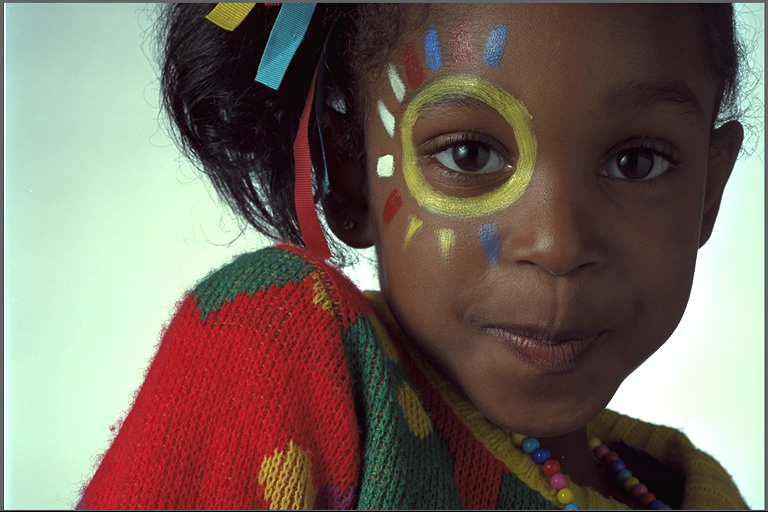
\includegraphics[width=0.4\textwidth]{out/15q65.jpeg}
        }\\
        \subfigure[Quality factor = 80]{%
            \label{fig:third}
            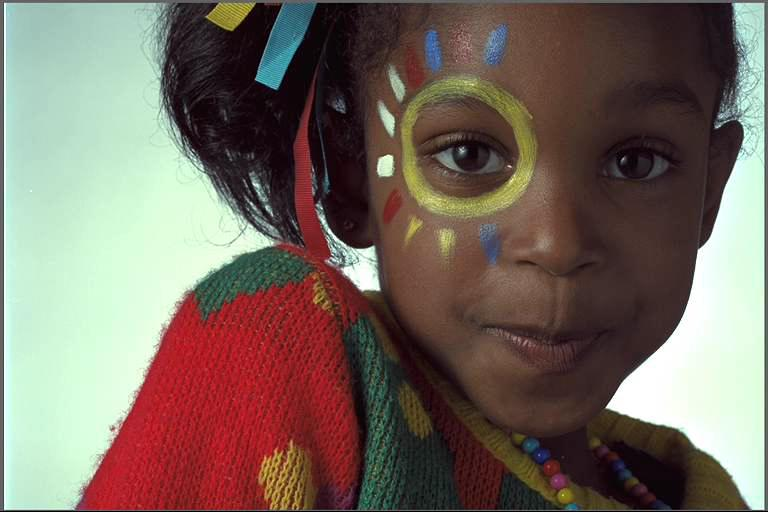
\includegraphics[width=0.4\textwidth]{out/15q80.jpeg}
        }%
        \subfigure[Quality factor = 100]{%
            \label{fig:fourth}
            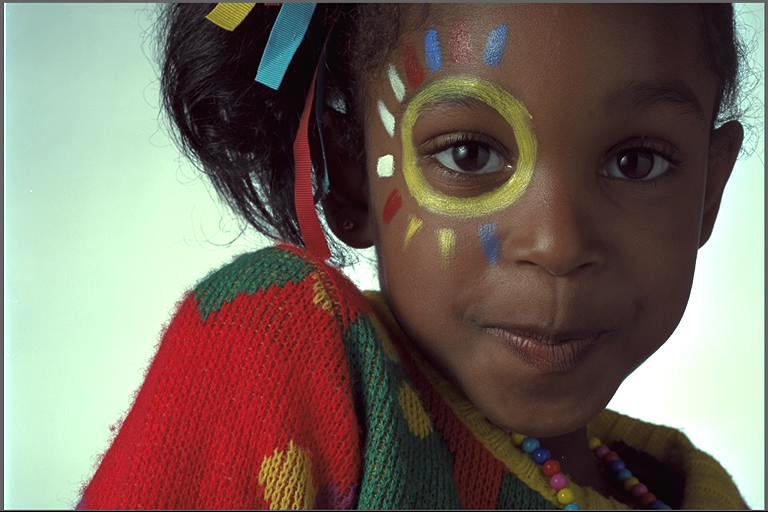
\includegraphics[width=0.4\textwidth]{out/15q100.jpeg}
        }%
%
    \end{center}
    \caption{kodim15.png}
\end{figure}

\begin{figure}[H]
     \begin{center}
%
		\subfigure[Original]{%
            \label{fig:first}
            \includegraphics[width=0.25\textwidth]{dataset/kodim19.png}
        }%
        \subfigure[Quality factor = 5]{%
            \label{fig:first}
            \includegraphics[width=0.25\textwidth]{out/19q5.jpeg}
        }%
        \subfigure[Quality factor = 15]{%
           \label{fig:second}
           \includegraphics[width=0.25\textwidth]{out/19q15.jpeg}
        }\\
        \subfigure[Quality factor = 30]{%
            \label{fig:first}
            \includegraphics[width=0.25\textwidth]{out/19q30.jpeg}
        }%
        \subfigure[Quality factor = 50]{%
            \label{fig:third}
            \includegraphics[width=0.25\textwidth]{out/19q50.jpeg}
        }%
        \subfigure[Quality factor = 65]{%
            \label{fig:fourth}
            \includegraphics[width=0.25\textwidth]{out/19q65.jpeg}
        }\\
        \subfigure[Quality factor = 80]{%
            \label{fig:third}
            \includegraphics[width=0.25\textwidth]{out/19q80.jpeg}
        }%
        \subfigure[Quality factor = 100]{%
            \label{fig:fourth}
            \includegraphics[width=0.25\textwidth]{out/19q100.jpeg}
        }%
%
    \end{center}
    \caption{kodim19.png}
\end{figure}

\section{Conclusions}
As seen in the previous section, my approach to the JPEG coding scheme gives results not too far from the standard algorithm in terms of visual quality and PSNR, even though the compressed image size is always bigger. Despite the gain obtained by the chroma subsampling method, the most significative difference between the two implementations is given in terms of computational complexity. Some optimizations could be applied to my algorithm mainly in the coding part, possibly by encoding separately the quantized DC and AC coefficients obtained by the DCT.

This project has been stimulating to develop in many ways. For the practical point of view, it was challenging to work with the MATLAB tools for encoding and for block-oriented programming with \texttt{blocproc}, which I was new to. Furthermore, it was interesting to discuss the results as I learned how fine a compression process can be and how many parameters there exist to evaluate the quality of a certain compression.

\end{document}